\subsection{FoodProcessor}
	The FoodProcessor's responsibility is to generate a random position for food placement. The FoodProcessor class is used when the snake collides with currently placed food, where a new position is the generated. Figure \ref{fig:classFood} shows a class diagram of the FoodProcessor.

		\begin{figure}[H]
			\centering
			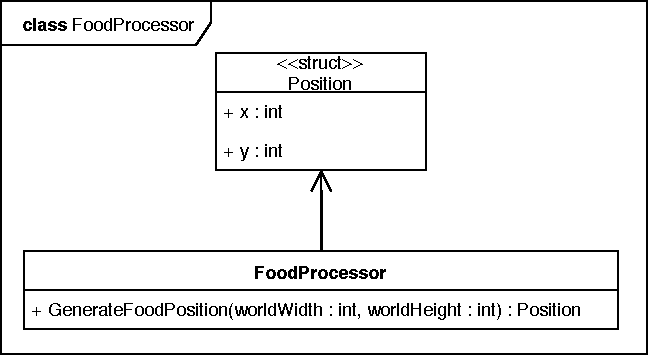
\includegraphics[scale=1.0]{FoodProcessorClassDiagram}
			\caption{Class diagram for FoodProcessor}
			\label{fig:classFood}
		\end{figure}
		
	The figure shows that the new position is wrapped in a Position struct which contains the x and y values. The parameters for the single function in the FoodProcessor are the constraints to the generated Position.	